\documentclass{tufte-book}

\hypersetup{colorlinks}% uncomment this line if you prefer colored hyperlinks (e.g., for onscreen viewing)

%%
% Book metadata
\title{MvdMlab Manual}
%\author[MvdM]{MvdM}
%\publisher{Publisher of This Book}

%%
% If they're installed, use Bergamo and Chantilly from www.fontsite.com.
% They're clones of Bembo and Gill Sans, respectively.
%\IfFileExists{bergamo.sty}{\usepackage[osf]{bergamo}}{}% Bembo
%\IfFileExists{chantill.sty}{\usepackage{chantill}}{}% Gill Sans

%\usepackage{microtype}

%%
% For nicely typeset tabular material
\usepackage{booktabs}

%%
% For graphics / images
\usepackage{graphicx}
\setkeys{Gin}{width=\linewidth,totalheight=\textheight,keepaspectratio}
\graphicspath{{graphics/}}

% The fancyvrb package lets us customize the formatting of verbatim
% environments.  We use a slightly smaller font.
\usepackage{fancyvrb}
\fvset{fontsize=\normalsize}

%%
% Prints argument within hanging parentheses (i.e., parentheses that take
% up no horizontal space).  Useful in tabular environments.
\newcommand{\hangp}[1]{\makebox[0pt][r]{(}#1\makebox[0pt][l]{)}}

%%
% Prints an asterisk that takes up no horizontal space.
% Useful in tabular environments.
\newcommand{\hangstar}{\makebox[0pt][l]{*}}

%%
% Prints a trailing space in a smart way.
\usepackage{xspace}

% Prints the month name (e.g., January) and the year (e.g., 2008)
\newcommand{\monthyear}{%
  \ifcase\month\or January\or February\or March\or April\or May\or June\or
  July\or August\or September\or October\or November\or
  December\fi\space\number\year
}


% Prints an epigraph and speaker in sans serif, all-caps type.
\newcommand{\openepigraph}[2]{%
  %\sffamily\fontsize{14}{16}\selectfont
  \begin{fullwidth}
  \sffamily\large
  \begin{doublespace}
  \noindent\allcaps{#1}\\% epigraph
  \noindent\allcaps{#2}% author
  \end{doublespace}
  \end{fullwidth}
}

% Inserts a blank page
\newcommand{\blankpage}{\newpage\hbox{}\thispagestyle{empty}\newpage}

\usepackage{units}

% Typesets the font size, leading, and measure in the form of 10/12x26 pc.
\newcommand{\measure}[3]{#1/#2$\times$\unit[#3]{pc}}

% Macros for typesetting the documentation
\newcommand{\hlred}[1]{\textcolor{Maroon}{#1}}% prints in red
\newcommand{\hangleft}[1]{\makebox[0pt][r]{#1}}
\newcommand{\hairsp}{\hspace{1pt}}% hair space
\newcommand{\hquad}{\hskip0.5em\relax}% half quad space
\newcommand{\TODO}{\textcolor{red}{\bf TODO!}\xspace}
\newcommand{\ie}{\textit{i.\hairsp{}e.}\xspace}
\newcommand{\eg}{\textit{e.\hairsp{}g.}\xspace}
\newcommand{\na}{\quad--}% used in tables for N/A cells
\providecommand{\XeLaTeX}{X\lower.5ex\hbox{\kern-0.15em\reflectbox{E}}\kern-0.1em\LaTeX}
\newcommand{\tXeLaTeX}{\XeLaTeX\index{XeLaTeX@\protect\XeLaTeX}}
% \index{\texttt{\textbackslash xyz}@\hangleft{\texttt{\textbackslash}}\texttt{xyz}}
\newcommand{\tuftebs}{\symbol{'134}}% a backslash in tt type in OT1/T1
\newcommand{\doccmdnoindex}[2][]{\texttt{\tuftebs#2}}% command name -- adds backslash automatically (and doesn't add cmd to the index)
\newcommand{\doccmddef}[2][]{%
  \hlred{\texttt{\tuftebs#2}}\label{cmd:#2}%
  \ifthenelse{\isempty{#1}}%
    {% add the command to the index
      \index{#2 command@\protect\hangleft{\texttt{\tuftebs}}\texttt{#2}}% command name
    }%
    {% add the command and package to the index
      \index{#2 command@\protect\hangleft{\texttt{\tuftebs}}\texttt{#2} (\texttt{#1} package)}% command name
      \index{#1 package@\texttt{#1} package}\index{packages!#1@\texttt{#1}}% package name
    }%
}% command name -- adds backslash automatically
\newcommand{\doccmd}[2][]{%
  \texttt{\tuftebs#2}%
  \ifthenelse{\isempty{#1}}%
    {% add the command to the index
      \index{#2 command@\protect\hangleft{\texttt{\tuftebs}}\texttt{#2}}% command name
    }%
    {% add the command and package to the index
      \index{#2 command@\protect\hangleft{\texttt{\tuftebs}}\texttt{#2} (\texttt{#1} package)}% command name
      \index{#1 package@\texttt{#1} package}\index{packages!#1@\texttt{#1}}% package name
    }%
}% command name -- adds backslash automatically
\newcommand{\docopt}[1]{\ensuremath{\langle}\textrm{\textit{#1}}\ensuremath{\rangle}}% optional command argument
\newcommand{\docarg}[1]{\textrm{\textit{#1}}}% (required) command argument
\newenvironment{docspec}{\begin{quotation}\ttfamily\parskip0pt\parindent0pt\ignorespaces}{\end{quotation}}% command specification environment
\newcommand{\docenv}[1]{\texttt{#1}\index{#1 environment@\texttt{#1} environment}\index{environments!#1@\texttt{#1}}}% environment name
\newcommand{\docenvdef}[1]{\hlred{\texttt{#1}}\label{env:#1}\index{#1 environment@\texttt{#1} environment}\index{environments!#1@\texttt{#1}}}% environment name
\newcommand{\docpkg}[1]{\texttt{#1}\index{#1 package@\texttt{#1} package}\index{packages!#1@\texttt{#1}}}% package name
\newcommand{\doccls}[1]{\texttt{#1}}% document class name
\newcommand{\docclsopt}[1]{\texttt{#1}\index{#1 class option@\texttt{#1} class option}\index{class options!#1@\texttt{#1}}}% document class option name
\newcommand{\docclsoptdef}[1]{\hlred{\texttt{#1}}\label{clsopt:#1}\index{#1 class option@\texttt{#1} class option}\index{class options!#1@\texttt{#1}}}% document class option name defined
\newcommand{\docmsg}[2]{\bigskip\begin{fullwidth}\noindent\ttfamily#1\end{fullwidth}\medskip\par\noindent#2}
\newcommand{\docfilehook}[2]{\texttt{#1}\index{file hooks!#2}\index{#1@\texttt{#1}}}
\newcommand{\doccounter}[1]{\texttt{#1}\index{#1 counter@\texttt{#1} counter}}

% opening quotes (from https://tex.stackexchange.com/questions/53377/inspirational-quote-at-start-of-chapter)
%\usepackage{epigraph}
\makeatletter
\renewcommand{\@chapapp}{}% Not necessary...
\newenvironment{chapquote}[2][2em]
  {\setlength{\@tempdima}{#1}%
   \def\chapquote@author{#2}%
   \parshape 1 \@tempdima \dimexpr\textwidth-2\@tempdima\relax%
   \itshape}
  {\par\normalfont\hfill--\ \chapquote@author\hspace*{\@tempdima}\par\bigskip}
\makeatother

% Generates the index
\usepackage{makeidx}
\makeindex

\usepackage{color}
\definecolor{lightgray}{gray}{0.75}

\newcommand\greybox[1]{%
  \vskip\baselineskip%
  \par\noindent\colorbox{lightgray}{%
    \begin{minipage}{\textwidth}#1\end{minipage}%
  }%
  \vskip\baselineskip%
}

\usepackage[parfill]{parskip}
\setlength{\parindent}{0pt} % hmm neither of these options get rid of
                            % the indent! -- MvdM

\begin{document}

% Front matter
%\frontmatter

% r.1 blank page
%\blankpage

% v.2 epigraphs
%\newpage\thispagestyle{empty}
%\openepigraph{%
%A designer knows that he has achieved perfection 
%not when there is nothing left to add, 
%but when there is nothing left to take away.
%}{Antoine de Saint-Exup\'{e}ry}
%\vfill

% r.3 full title page
\maketitle

% r. 4 copyright and attributions
\newpage
\begin{fullwidth}
~\vfill
\thispagestyle{empty}
\setlength{\parindent}{0pt}
\setlength{\parskip}{\baselineskip}
Copyright \copyright\ \the\year\ van der Meer lab

\par\smallcaps{www.vandermeerlab.org}

\begin{figure}
  \includegraphics[width=5cm]{images/license.png}
%  \checkparity This is an \pageparity\ page.%
\end{figure}


\par Licensed under the Creative Commons BY-NC-SA License (the
``License''), version 4.0; you may not use this file except in
compliance with the License. Briefly, you are free to share and adapt
this material, under the condition that you give appropriate credit,
do not use the material for commercial purposes, and distribute your
contributions under the same terms. You may obtain a copy of the full
License at \url{https://creativecommons.org/licenses/by-nc-sa/4.0/}.

\par Inspired by similar lab manuals by others. Particularly helpful
were the wonderful examples from the
\href{http://jpeelle.net/peellelab_manual.pdf}{Peelle} and \href{https://github.com/alylab/labmanual}{Aly} labs.

\par Typeset in Palatino Linotype using \LaTeX{} and the
\doccls{tufte-book} class.

\par\textit{Version 0.1, \monthyear}
\end{fullwidth}

% r.4 contents
\setcounter{tocdepth}{1}
\tableofcontents

% r.9 introduction
\chapter{Welcome!}

\begin{chapquote}{Luna, {\it Double Feature} (1995)}
I didn't change my mind, it changed all by itself.
\end{chapquote}

\newthought{The van der Meer lab} brings together people who share an
interest in how the brain works. We aim to better understand how
learning, memory, and decision-making arise from the coordinated
activity of neurons. In the pursuit of this goal, we perform brain
surgery, design and construct strange mazes, painstakingly build small
devices so we can read the minds of rats, solder tiny circuit boards
to even tinier wires, write thousands of lines of computer code,
collect beautiful data, produce even more beautiful plots, and many
other activities.

\begin{marginfigure}[-4cm]
\centering{
\includegraphics[width=0.7\linewidth]{images/shortcut_mazes.png}
}
\caption{Some strange mazes. (From Emily Irvine's {\it shortcut} experiment.)}
\label{fig:shortcut}
\end{marginfigure}

\newthought{Each of us brings} their own particular blend of
motivations for engaging in these lab activities, but there are a few
common threads: curiosity about how the physical stuff of the brain
gives rise to thought and to behavior, a love for animals and
computers alike, a desire to help solve some of the big mysteries, and
contributing to human knowledge and ultimately a better world.

\begin{marginfigure}[3cm]
\centering{
\includegraphics[width=0.7\linewidth]{images/8tt_drive.png}
}
\caption{A small device for rat mind-reading (by Andrew Alvarenga).}
\label{fig:8tt_drive}
\end{marginfigure}

\newthought{Our efforts are {\it collaborative}}, not only within the
lab, but also with other labs in the department of Psychological \&
Brain Sciences at Dartmouth. We share equipment, space, and interests
with these labs, and collaborate on joint projects and on creating a
scientifically exciting and supportive culture where everyone can
thrive. We also have joint projects with other labs around the
world. We collaborate because the problems we are trying to solve are
hard, and because learning from and working with others is one of the
great joys of working in science!

\newthought{Working with others} brings not only joy, but also
expectations. Coding and data analysis can be fun, but are full of
pitfalls. Sharing space and expensive equipment with others demands
respect. There is satisfaction in getting an experiment to work, but
it can be a long slog to get there. Perhaps most importantly of all,
the use of animals in research comes with practical as well as moral
responsibilities. {\it This manual is intended to provide guidance on how
to navigate these issues, with particular focus on the van der Meer
lab.}

\begin{marginfigure}
\centering{
\includegraphics[width=\linewidth]{images/R050_raster.png}
}
\caption{Some beautiful data, recorded from R050's hippocampus (by
  Alyssa Carey). Vertical tick marks indicate spikes (one row per
  neuron, sorted by place field location); horizontal axis indicates
  time; blue trace shows a local field potential. Scale bar is 1 s.}
\label{fig:raster}
\end{marginfigure}

\newthought{If you are new to the lab}, I would like you to read this
manual through in its entirety. If you will not be working with
animals directly, it may seem like chapter on
\hyperref[sec:animal-management]{Animal Management} does not apply to
you, but it will give you important insights into how the lab
operates.

\newthought{Welcome}. Let's do some great science together!

\begin{chapquote}{{\it MvdM}}
\end{chapquote}
%%
% Start the main matter (normal chapters)
\mainmatter

\chapter{About this manual}

\newthought{This document} describes the principles that shape how the
members of the lab interact and work. Rather than dealing with the
nuts and bolts of how to get stuff done in the lab, the manual is
about lab philosophy, expectations, and resources. It is an
introduction to the lab. The lab manual is one of several classes
(categories) of shared documents in the lab, which are:

\begin{itemize}
\item{{\it Lab Manual}. You are looking at it. It contains information
  that does not change frequently. Only MvdM can change the lab
  manual, but he wants to hear from you if you have thoughts of
  suggestions! Periodically, we will review the manual as a group at
  lab meeting to determine what needs updating.}
\item{Private {\it GitHub
    repositories}\sidenote{\url{www.github.com/vandermeerlab}. Because
    these repositories are private, you will not be able to see them
    unless you are logged in and a member of the vandermeerlab
    organization.} that contain \doccls{protocols},
  i.e.\ documentation for experimental procedures\sidenote{Examples
    include electrode plating, histology, drive building, et cetera:
    \url{mvdmlab-protocols} repository}, and a separate repository for
  \doccls{behavioral tasks} and associated computer
  code\sidenote{\url{mvdmlab-tasks}}. This documentation is on GitHub
  so that we can say things like, ``I used version 1.1 of the histology
  protocol'', and so that we can track changes to those protocols as
  well as the reasons for those changes. If you perform procedures in
  the lab, you are expected to follow and to contribute to these
  protocols; see section XXX for a more detailed explanation.}
\item{A {\it lab
    wiki}\sidenote{\url{discovery.dartmouth.edu/~mvdm/wiki}} that
  contains tutorials, guides, lists of useful links, et cetera. The
  wiki is a more dynamic, easier to edit resource for content that
  doesn't rely as much on version control. The wiki currently contains
  the lab's MATLAB data analysis tutorials.}
\item{We also have a lab {\it Slack}
  team\sidenote{\url{mvdmlab.slack.com}} which is used for day to day
  communication. It hosts shared documents best described as
  ``everything else'', something that isn't a protocol, task, or
  tutorial.}
\end{itemize}

These different venues reflect an overall organization ranging from
content that is easy to create and easy to change (low overhead,
quick; Slack, wiki), to content that is moderately stable and takes a
bit more effort to change (but easier to track; GitHub), to principles
that rarely change (lab manual). For instance, an idea for an
experiment may be initially discussed on Slack, lead to a draft
protocol shared there, and then get pushed to GitHub. 

There are a number of other kinds of documents used in the lab that,
unlike the above categories, are not typically consulted by multiple
lab members. Most important among these are (1) animal records,
described in more detail in section XXX, and (2) lab notebooks,
described in section YYY. 

\greybox{
\textsf{I assume the lab manual and procedures on GitHub are
  accurate. This means that you should follow all of the policies and
  procedures contained in the manual and GitHub. If you notice
  something that seems to be wrong, please let me know (for the lab
  manual) or change it yourself (if on GitHub). If there is something in
  the lab manual or GitHub that you notice people aren't doing, please
  bring this up at lab meeting, or to me directly. Don't assume this
  is okay (it's not).}}

%%% RESEARCH USING ANIMALS &&&
\chapter{Research Using Animals}
\label{ch:animals}

\newthought{We use animals} in the lab, based on the conviction that
doing so accelerates scientific progess and provides a net benefit to
humans, and perhaps to animals, too. There are many examples of
scientific discoveries that were directly enabled by resarch in
animals\sidenote{Some good examples include the ``Position statement
  of the Max Planck Society concerning the use of animals in
  experiments for basic research'',
  \url{https://www.mpg.de/10882259/MPG_Whitepaper.pdf}}. However,
these successes do not mean we can experiment freely on any animal we
want. The use of animals for research carries a moral, scientific, and
legal obligation to only perform experiments where the benefits
outweigh the costs, where no suitable alternatives are available, and
to care for our animals to the fullest extent possible. These notions
are often phrased as the ``3 R's'' (reduction, replacement,
refinement)\sidenote{Some references on the 3 Rs}.

More generally, research in animals demands that we do the best job
possible, and maximize the usefulness of the research outcomes.

This means that:

\begin{itemize}
\item{We take care of our animals. If animals are comfortable and well
  cared for, they will perform the behavioral tasks we want, be easy
  to handle.}
\item{We strive to design experiments so the outcomes will be as
  informative as possible.}
\item{We aim to collect the highest quality data possible.}
\item{For the data to be interpretable, good records need to be kept.}
\item{Data is valuable. It needs to be protected, and be easy to
  use. This means it needs to be organized and annotated in a specific
  common format.}
\end{itemize}

In sum, the fact we are working with animals shapes both our lab
philosophy and many practical aspects of working in the lab.

\begin{marginfigure}
\centering{
\includegraphics[width=0.9\linewidth]{images/rat_with_objects.png}
}
\caption{A cartoon rat with some objects. Figure from Dudchenko et al.}
\label{fig:rat-with-objects}
\end{marginfigure}

Doing research with animals shapes not only the philosophy of the lab,
but also has pervasive consequences for day-to-day work. Later
sections of this manual, such as XXX and YYY, will deal in more detail
with the nuts and bolts.

All of these components will be discussed on more detail in the
relevant sections. This chapter is intended to provide some key
definitions, references, and principles.

Animal research at Dartmouth is overseen by the IACUC.

All work with animals (specifically, all procedures) needs to receive
prior approval from the IACUC in the form of
{\it protocols}\sidenote{{\it Protocol}: document outlining the
  scientific rationale, aims, and a set of proposed experiments.}.

Animal care is provided by CCMR.

At a minimum, we are required to log all {\it
  procedures}\sidenote{{\it Procedure:} Any action or change beyond
  picking an animal up in the colony room (e.g.\ for changing cages or
  weighing) counts as a procedure}.

Apart from the moral obligation to care for our animals and ensure
they can contribute to science, we often invest a tremendous amount of
time in each animal through behavioral training, construction of
chronic implants, surgery, and so on. If any one of these procedures
is not performed diligently, then your investment in all the others
may come to nothing.

%%%%%%%%%%%%%%%%%%%%
%%% EXPECTATIONS %%%
%%%%%%%%%%%%%%%%%%%%

\chapter{Values and Expectations}\label{ch:expectations}

The lab values personal and scientific integrity, respect for each
other, for animals, for equipment, and for data. We care about shaping
and maintaining an environment that fosters personal development,
curiosity, exploration, and the joy of discovery. We choose to work on
hard problems that require dedication, persistence, resourcefulness,
and resilience. We are humble. We support each other in when things
get tough, and celebrate each other's successes. We value
opportunities to learn from each other, set high standards but do not
judge.

Holding these values implies the following:

\section{Expectations: everyone}

\begin{itemize}
\item{Take initiative. If you are stuck, try something different. Ask
  someone.}
\item{Document. Anything you do more than once, or that you or someone
  else might have to do again, should be written up as a
  \doccls{protocol}. Anything done with an animal is a
  \doccls{procedure} and needs to be logged. Good recordkeeping is
  essential to doing good science. Keep track of what you did with
  experiments and analyses in your \doccls{lab notebook}.}
\item{Communicate. Tell others what you are working on, what is
  working well and what could be improved. Post on updates on Slack
  frequently.}
\item{Contribute to community resources and space. If you notice
  something that can be improved, fix it, mention it on Slack, or open
  a GitHub issue.}
\item{Collaborate. Share your expertise. Make arrangements with others
  to take care of their animals one weekend and reciprocate
  another. Offer to do code reviews, read each other's manuscript,
  offer feedback on practive talks.}
\item{Showing up. There will be days when it feels like you aren't
  making any progress and nothing is working. Don't underestimate the
  power of an iterative routine.}
\item{Be a little obsessive.}
\item{Be punctual.}
\item{Take care of yourself. Know when it's time to push, and when
  it's time to take a walk in Pine Park\sidenote{See here for a guide
    to some of Hanover's best trails, accessible from the lab in the
    space of a lunch break.}.}
\item{Tell others when you notice they did something well, or when
  they made your life a little better today\sidenote{We have the
    \doccls{octothorp}, awarded during lab meeting. But don't stop
    there!}.}
\item{Keep at it. While brilliant ideas, creativity and skill
  certainly help, the best predictor of success is how consistently
  you put in the work.}
\end{itemize}

Values: personal and scientific integrity; respect for animals,
humans, equipment, data, space. Supportive and collaborative learning
atmosphere that fosters personal development, curiosity, exploration,
joy of discovery. For this to count, need persistence, resilience, and
hard work. This is only possible if you are pursuing something you
care about, and take care of yourself and those around you (so they
may reciprocate). Be kind. Non-judgmental, recognize that failing
often is part of science, changing your opinion is better than having
no opinion.

Well-being. Work hard but be kind to yourself and others.

Share your expertise, be respectful of others' time.

Attend weekly lab meetings.


% pi
\section{Principal Investigator}

Have a vision for where the lab is going, and how to get there.

Provide an environment where great science can be done and people can thrive.

Obtain funding.

Help train you.

\section{Graduate Students}\label{sec:gradstudents}

Make an original contribution to knowledge.

% techs
\section{Research Technicians}


% ugrad
\section{Undergraduates}

Onboarding process.

Letters of recommendation.

Funding sources for research and travel.


\section{Code of Conduct}

Short version: be nice. Science needs contributions from
everyone. There are well-documented barriers to participating that we
want to do our best to help eradicate.

Some specific things that work well:

Long version: laid out in Dartmouth policies.

\chapter{Doing good science}

This chapter provides some general strategies that effective
scientists use.

\section{Failing fast and often, but learn from your mistakes}

Science involves a lot of trial and error. You will be asking
questions whose answers are often not yet known, using combinations of
techniques and analyses that do not yet exist or have not been applied
to your particular question. So you want to find ways to learn from
errors as quickly as possible, and ways to avoid making them in the
first place.

The general principle to do this is to find ways to get feedback
often. For projects that are at the idea stage, talk with your peers
about it, and solicit feedback from more senior colleagues. Find out
what the likely pitfalls and challenging steps are, and who has
already tried or even solved them before.

For projects that are experimental, the same idea applies: find a
setup in which the feedback cycle is as short as it can be. For
instance, if your project requires recording from a brain area that
the lab has not recorded from before, chronically implanting an animal
would take much longer until you find out if you hit, compared to
doing an acute (non-recovery) surgery.

Experiments often consist of multiple steps or components that all
need to work -- failure in any component will make all the other steps
in vain\sidenote{A typical example is that if you do not follow
  aseptic surgical procedures, an infection may cause your implant to
  detach. Having built perfect electrodes is then moot.}. This implies
that you should find ways to get feedback about whether each component
is working correctly. For instance, inspect your tetrodes under a
microscope before attaching them to the interface board.

For analysis projects, a similar logic again applies: formulate
expectations about what the output of a given analysis step should
look like. 

For all of these processes, apply a hacker/startup mindset that takes
the quickest path towards a minimal working example or proof of
principle. At that point, if the results look promising, you should
clean up, improve and document things.

Often, things will not work. This is not always a problem -- sometimes
you just want to try something and only follow up if it looks like
things are going to work. However, some failures actually block your
way forward, and you will need to resolve them. Notes, as described
next, will help you (and others) identify what the problem might
be. Making the same mistake twice is not a good use of time and
resources.

\section{Documentation and taking good notes}

One way to avoid making the same mistake twice or to avoid making them
in the first place is to have good documentation.

A related but different reason to care about documentation is that a
desirable property of a scientific study is that it should be possible
for others to replicate the result.

\subsection{Lab notebook}

\subsection{Protocols}

Protocols are step-by-step instructions of procedures used in the
lab. Anything you expect to do again in the future should be written
up as a protocol. If you only do a thing once, you should still take
notes!

Protocols are hosted on GitHub. Why?

What makes a good protocol? Use standard structure (purpose,
ingredients, equipment). Step-by-step instructions: it should be a
recipe, and algorithm. The main procedures should be clean and minimal
so that it is easy to get an overview, but adding copious notes and
explanations as footnotes/sidenotes/appendices are great. Steps should
be as easy as possible to follow, with checks/tests that can be used
to tell if things are working as expected. Pictures can be very
helpful here.

Some example protocols are:

If you use a protocol, update it regularly, even if it is to say when
it was last used successfully (and by whom).


\section{Asking good questions}

{\it Questions about science.}

Experiments and analyses are ways of asking nature a question. Your
goal should never be to obtain a certain answer. You should formulate
expectations about possible answers and consider if those would in
fact inform the question you are asking.

Working models are good sources of questions.

{\it Questions about computer code.} 

When troubleshooting computer code, aim to create a \doccls{Minimal,
  Complete, and Verifiable example}. In doing so, you make it easier
for others to replicate the problem you are experiencing, helping them
help you. Moreover, often you'll find that in the process of creating
such an example, you discover the source of the problem. See
\href{https://stackoverflow.com/help/mcve}{this page} on Stack
Overflow\sidenote{\url{www.stackoverflow.com}, an excellent resource
  for crowdsourced answers to programming issues.} for more detailed
instructions.


\section{Reading papers}

Inspectional, analytical, syntopical

Bibliography management

Find the classic papers and intellectual roots of the question you are
working on. If this doesn't motivate or energize you at least from
time to time, ask yourself how much you actually care about your question.

\section{Communication}

\subsection{Writing well}

Clear thesis

Structure of argument

Vomit draft, results packet

Iterating often

Citing: first, best, and most recent (this is a good rule of thumb to
guide your reading, too.)

Simpler is better

See SOFTWARE SECTION for more info on recommendations.

\subsection{Importance of visuals}

Simpler is better

See SOFTWARE SECTION.

%%%%%%%%%%%%%%%%%%
%%% FACILITIES %%%
%%%%%%%%%%%%%%%%%%

\chapter{Lab space}

Our lab space consists of the following:

Include map.

\section{General expectations}

In the lab, we assemble precision devices that will be surgically
implanted in live animals. We perform behavioral experiments that are
sensitive to changes in many different conditions. The amount of time
invested in these procedures, and the fact that we are doing this in
live animals, demand careful attention. In addition, lab space is
subject to general lab safety requirements (link) and IACUC
inspections (link).

The principle that guides the use of shared lab space is that any lab
member needs to be able to come in, find the items they need, and get
things done to a high standard. In addition, the condition in which te
lab spaces are kept should reflect pride taken in doing good work --
it will be seen and interpreted by others viewing our space.
Depending on the specific rooms this can mean somewhat different
things, discussed in more detail below, but there are some common
principles:

\begin{itemize}
\item{{\it Clean up after yourself}. Use common sense about when to do
  this. If you're in the middle of something and stepping out to get
  some lunch, it makes no sense to clear your work area. However, if
  you've finished what you were working on, definitely clean
  up. Before going home for the day is usually a good time to at least
  clean a bit. See the specific room schedules for more specific
  cleaning requirements.}
\item{{\it Organize where things are stored}. Any item in the lab has a
  home. Some individual items are sufficiently important that they
  have a dedicated place, such as ``final cut scissors''
  (PICTURE). Some items don't have a dedicated place but are a member
  of a more general category, such as ``BNC interconnects''. If you
  find an item that does not have an obvious home, check on Slack if
  anyone has suggestions, and/or create one for it. Creating a home
  for an item can be as simple as labeling a piece of a shelf
  somewhere. Make sure you tell everyone about it on Slack, in
  accordance with the Communication Principle!}
\item{{\it Track stock levels.} If something is running low, don't
  just ignore it. Post about it on Slack. Store parts that go with a
  certain piece equipment with that equipment (for instance, by taping
a ziploc baggie to it).}
\item{{\it Label things.} Any liquid and food containers MUST be labeled with
  the contents and expiry date, if applicable. When you open a new
  package of something, write on it when you opened it. When a new
  thing comes in, write on it when it was received.}
\item{{\it Treat tools with respect.} What may look like a cheap pair of
  scissors is likely to cost at least \$300. Use tools for their
  intended purpose, and use the correct tool for the job. For
  instance, don't use fine scissors to make rough cuts into hard
  materials. Don't use fine forceps to hold metal parts. \sidenote{Quick
  guide to forceps: \#55 are finest.}}
\item{{\it Be safe.} The general lab safety training covers the
  basics, but specific spaces have hazards described below. First Aid
  kits are available in the FAR and in B101.}
\end{itemize} 


\section{Experiment rooms}

AKA ``running rooms''

These are the main spaces that our rats interact with. That has a few
consequences:

\begin{itemize}
\item{If you have a rat out, have the doors closed. Put a sign on the
  door saying, ``Experiment in Progress''.}
\item{Don't make changes to the layout of the room while you are
  running an experiment. Changing the cues and landmarks available can
  change what strategy animals use to solve a behavioral task.}
\item{Work to keep light levels, sound levels, and odor cues
  consistent.}
\item{Any surface rats interact with needs to be cleanable. So, no
  cardboard, unsealed wood, and so on.}
\item{Our IACUC protocols require cleaning apparatus at least weekly.}
\end{itemize}

Cleanliness and organization is important, but don't let that hold you
back in shaping your workspace to enable you do perform your
experiments well and efficiently. Tape procedures you are using to the
walls, print out the relevant atlas sections, make temporary storage
spaces for the tools you use frequently.

\section{Fine Assembly Room (FAR)}

\section{Surgery and anteroom}

If there is any single room that is especially important to be clean
and organized, this is it!

\section{Workshop}

Beware the Dremel and the belt sander. Wear gloves and goggles.

\section{Shared facilities}

Histology.

\section{Vivarium space}

Our room is...

\section{Offices}


%%%%%%%%%%%%%%%%%%
%%%
%%%%%%%%%%%%%%%%%%
\chapter{Electronic resources}

\section{Dropbox, Drive, Calendar}

\section{GitHub}

\section{Slack}

\href{Slack}{www.slack.com} is a software platform for having group
conversations in topic-specific channels. The lab Slack is
\url{mvdmlab.slack.com}.

\begin{marginfigure}%
  \includegraphics[width=\linewidth]{images/slack.png}
  \caption{Slack.}
  \label{fig:slack}
\end{marginfigure}

\section{Wiki}

\section{Mailing list}

%%%%%%%%%%%%%%%%%
%%% COMPUTING %%%
%%%%%%%%%%%%%%%%%
\chapter{Computing}

Computing plays an increasingly important role in (neuro)science and
is central to many aspects of the lab's workflow. The safety of your
hard-won data, the integrity and reproducibility of your analyses and
results, the ongoing development and sharing of the best protocols and
procedures, and the speed with which you can accomplish your goals all
depend critically on correct use of the lab's computing resources.

Because many of these are shared (experimental machines) and/or
inherently collaborative (lab database, codebase) it is especially
important to be aware of the issues below. Experience with some of the
more advanced concepts and tools is a highly valued skill in many labs
and workplaces; mastery of these will set you apart from many of your
peers.

\section{Lab computers}

The lab's computers are a mixture of custom builds (by MvdM), designed
for a particular role, and general-purpose workstations purchased from
Dartmouth Computing Services. The different roles determine the best
way to use each machine. The roles are:

a) single-user machines in offices, one for each grad student/tech/postdoc
b) shared machine in B28, for use with NanoZ and high-power scopr
c) shared machine in B101, for use with the 3D printer
d) shared experimental equipment machines: for recording in B18

\subsection{Single user machines (grad students and postdocs)}

One of these will be exclusively yours to use during your tenure in
the lab. You are free to install software and change settings to suit
your needs as long as any changes (1) do not interfere with the
machine's ability to support research, and (2) fall within the
Dartmouth Computing guidelines (link).

Single user machines have a boot drive (C:) for the operating system
and frequently used software. This is a fast SSD drive with limited
space, so be mindful of what you install here. Absolutely do not use
this drive for any documents or data.

Save your work and data files on the data drive (D:), because this is
automatically backed up using RAID (i.e. there are actually two
``mirrored'' hard disks which behave as one virtual disk). Run
RaidXpert's check utility periodically to ensure the health of the
RAID array.

\subsection{Shared machines}

Unlike the single user machines, when using the shared machine you
will need to consider how your actions affect other users. A few
guidelines:

\begin{itemize}
\item{If need to save your work, create a folder with your name on the Data
drive. Do not leave work or data files on the desktop. If you find
anything that's not supposed to be there on the desktop or anywhere
else, put it in the lost-and-found folder on the desktop.}
\item{Do not install any software, or change any software and system
settings, without discussing with MvdM first. Do not delete any files,
but place them in lost-and-found instead.}
\item{If you log in to web services, make sure you log out when you are
done.}
\end{itemize}

\subsection{Experimental machines}

The above considerations for shared machines apply. In addition:

\begin{itemize}
\item{If you acquire data for your project, use correct renaming and backup
procedure when you finish your acquisition session. This is absolutely
essential: data is expensive, and you individually and the lab as a
whole cannot afford to lose any of it, EVER. Do not leave data in the
acquisition folder.}
\item{If you encounter a potential data file or folder that is not yours
and seems lost, make an effort to find out whose data it might be.}
\item{NEVER delete anything that looks like it might be data, unless you are absolutely certain that it has been backed up correctly.}
\end{itemize}

2. All machines, even the single-user ones, use the mvdmlab
account.

3. Machines are distributed across physically different locations. To
facilitate communication and data sharing, we maintain a list with
machine names, MAC and IP addresses, and the network port they are
plugged in to. Remember to update this if anything changes.

To move data between machines, we use freeSSHd, Dropbox, and WinVNC.

4. Web services accounts

gmail: mvdmlab@gmail.com
dropbox: mvdmlab@gmail.com
skype: vandermeerlab (for contacting suppliers and other lab-related business)

PRINTING

Please be considerate when using the printer. Keeping an electronic
library of PDFs using an iPad, Dropbox and iAnnotate is a worthwhile
investment that will make it much easier to find papers and your
comments in the future, and will save a LOT of paper!

The recording computers both have local printers attached for
obtaining protocols and weight sheets.

6. If you see Windows updates to install on any machine, go ahead and
install them. If a computer needs rebooting because of updates and you
can do so safely, go ahead.

7. Use of University computers (which includes all lab computers) is
governed by the Guidelines on Use of Waterloo Computing and Network
Resources. These are generally common sense, and not overly long so
have a look.

\section{Skills}

Growth mindset.

Basic skills: learning about your filesystem, what makes sense to
store where

Learn to use the command line.

Learn to code. MATLAB and Python are the most important. In our
subfield of neuroscience, MATLAB is still the most used, but Python is
gaining ground.

Good coding practices.

Style guide.

Other important software: reference manager, LaTeX if you plan to
write a paper or a thesis. Adobe Creative Suite for making figures.

How to ask good questions. Stack Overflow on how to create a
\href{https://stackoverflow.com/help/mcve}{minimal, complete, and
  verifiable} example.

\section{Software}

In general, you should feel free use whatever software is the best
tool for the job\sidenote{...where ``best'' is defined as the
  intersection between the capabilities of the software itself,
  suitability for the task at hand, and the user's ability to use it
  correctly.}, and you should feel free to do so. However, there are
startup costs associated with learning how to use new software, and
the lab has built up expertise and resources in a number of software
packages that work well. Learning to use these software packages will
help you be productive in the lab, and will be applicable in other
settings as well.

\begin{marginfigure}
\centering{
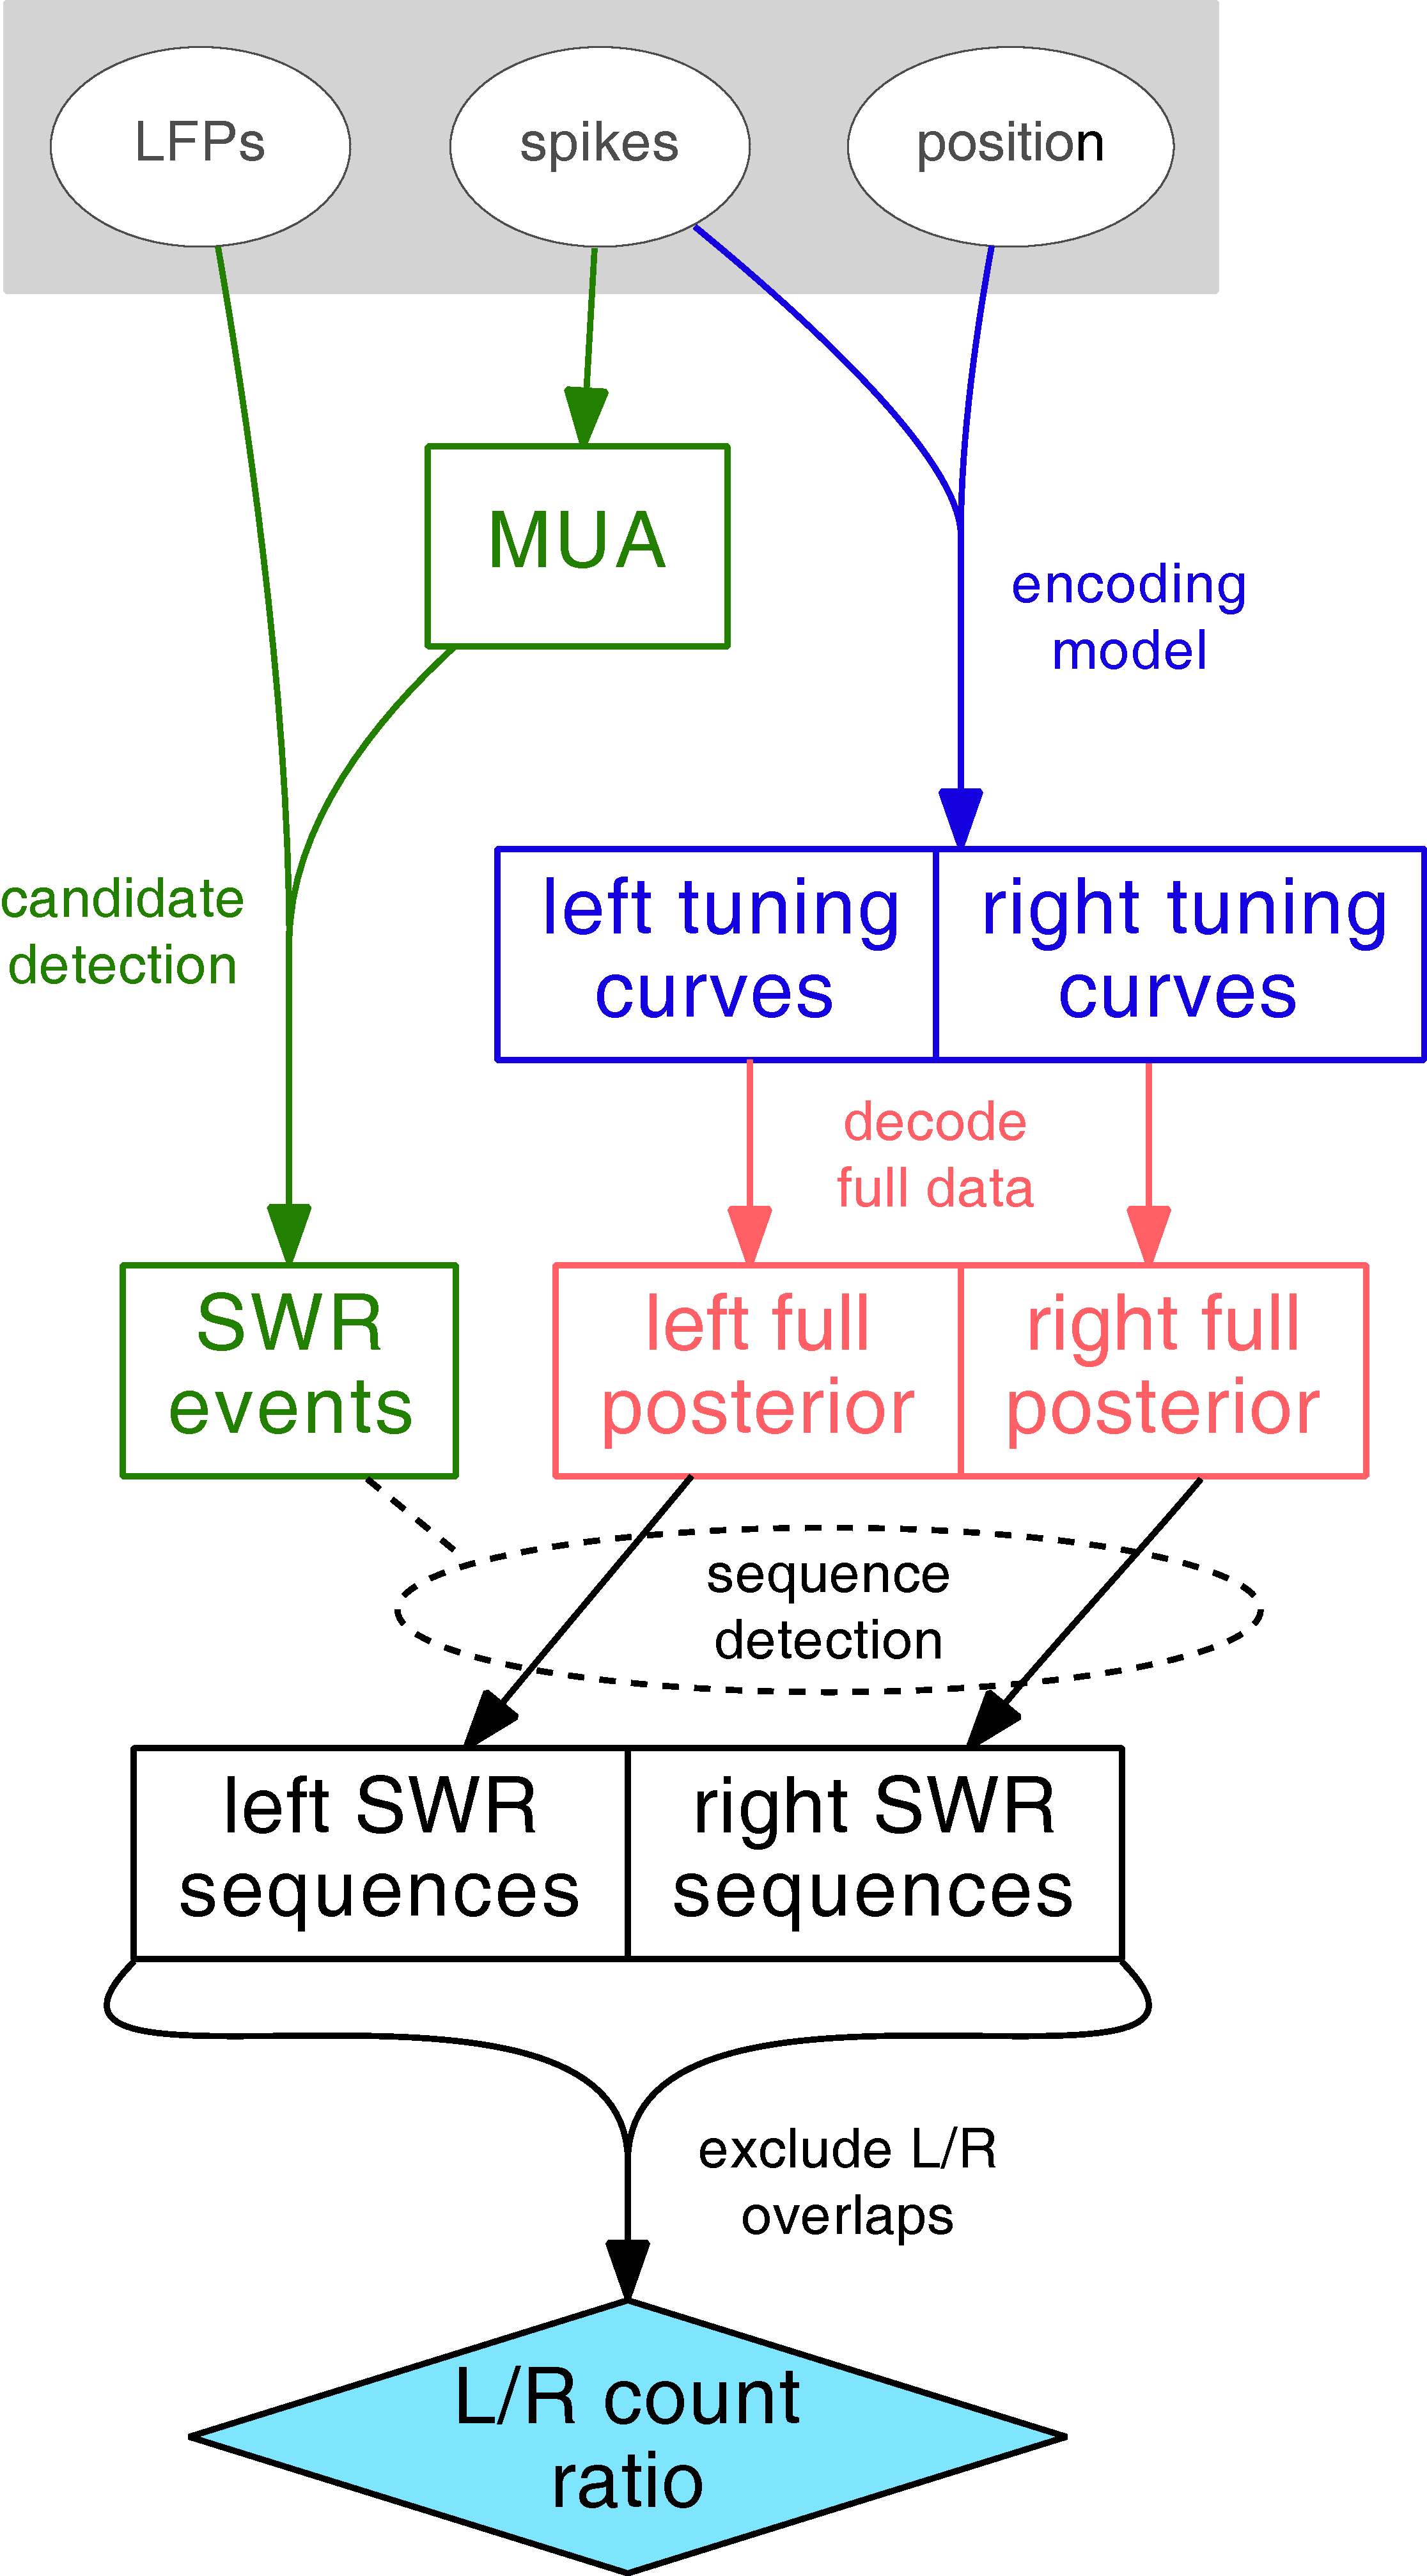
\includegraphics[width=\linewidth]{images/analysis_schematics.pdf}
}
\caption{Example data analysis workflow, made with \href{www.graphviz.org}{Graphviz}}
\label{fig:analysis-schematic}
\end{marginfigure}

\begin{itemize}
\item{{\bf Git} is a tool for ``collaborative version control'': a way
  to keep track of changes made to files such as computer code,
  experimental protocols or manuscrupt drafts, and to coordinate those
  changes across multiple contributors.}
\item{{\bf MATLAB} is a scientific computing environment that includes
  a programming language, libraries for performing specific tasks, a
  development environment with a fully featured editor, debugger, and
  interpreter, and many other features. It is widely used for data
  analysis in neuroscience. Although it is not free, Dartmouth has a
  site license that enables you to use it
  (\href{http://caligari.dartmouth.edu/downloads/matlab}{download
    page}). Python is becoming increasingly popular, and is far more
  widely used than MATLAB outside neuroscience. However, various
  toolboxes used in the lab such as Chronux and FieldTrip are still
  MATLAB-only, and MvdM is still a beginner in Python.}
\item{{\bf Adobe Creative Suite} is expensive, but produces superior
  documents. We use Illustrator to touch up and group together figure
  panels for manuscripts based on raw output from MATLAB or Graphviz,
  and to make posters. Photoshop is sometimes used to process image
  files such as those from histology. Free alternatives such as
  Inkscape and GIMP exist, can do the job for simple documents, but I
  don't (yet) recommend them for publication-quality output.}
\item{{\bf Graphviz} produces schematics such as the one in Figure
  \ref{fig:analysis-schematic}. Unlike
  `what-you-see-is-what-you-get'' design software such as Photoshop
  and Illustrator, the Graphviz tools create graphics from a plain
  text source file. The source file contains a recipe for what the
  graphic output should look like.}
\item{\LaTeX. Unlike ``what-you-see-is-what-you-get'' content creation
  programs such as Word, LaTeX creates documents from a plain text
  source file. The source file contains instructions for what the
  document should look like. Compared to Word, LaTeX does much better
  with equations, produces more professional-looking
  documents\sidenote{Especially where typesetting features such as
    spacing, kerning, and ligatures are concerned.}, and makes it much
  easier to maintain large documents.}
\end{itemize}

Note that several of these require you to use the Command Line
(Terminal).

\subsection{Operating Systems}

Lab computers use Windows and/or Ubuntu Linux. There are a few reasons
for this: the data acquisition machines require Windows (Neuralynx) or
Windows/Linux (Open Ephys), and custom machine builds are generally
cheaper for PCs than for Apple Macs. Nevertheless, many lab members
have Mac personal laptops that run OS X, and most of the above
software works fine on them. However, some Neuralynx loaders only work
on Windows, some codebase functions have only been compiled to work on
some OSes, and the lab only has licenses for some software (Adobe) to
work on Windows.

%%%%%%%%%%%%%%%%%%%%%%%%%
%%%% DATA MANAGEMENT %%%%
%%%%%%%%%%%%%%%%%%%%%%%%%
\chapter{Data management}

\newthought{Data is valuable.} After taking into account the number of
hours that went into training an animal, building a hyperdrive,
preparing for and performing surgery, painstakingly turning
electrodes; animal housing costs, costs of parts and consumables, and
so on, the cost of a single subject worth of data can run into tens of
thousands of dollars -- and this is without the moral calculation of
considering an animal's life. Data therefore needs to be treated with
the greatest respect: specifically, it needs to be managed so that it
can be maximally useful. The {\it first requirement} of data
management is that data needs to be available -- i.e.\ backed up so
that it can never be lost, and accessible by those who need it. Our
lab is committed to \doccls{Open Science}, of which public data
sharing is one component. Increasingly, journals and funders demand
that data is made publicly available. The {\it second requirement} of
data management is that the data needs to be organized such that it
can be easily understood and used.

Before discussing how these two requirements -- data storage and data
organization -- are implemented in the lab, it is useful to
distinguish between different categories of data.

\begin{itemize}

\item{{\bf Raw data} is what gets saved on a data acquisition machine,
  such as a running room computer connected to a Neuralynx recording
  system, or a machine connected to a microscope. Depending on the
  data you collect, a single session may yield many different files,
  such as behavioral tracking data and neural recording data, or a
  single file (an image). Raw data is only rarely suitable for
  analysis beyond a few quick checks. At a minimum, freshly acquired
  data sets typically must be annotated, and/or the files
  systematically renamed -- for instance, with the ID of the
  experimental subject and some information about recording locations
  -- so that the analyst can select which files to analyze, and combine
  results across sessions and subjects. More complex pre-processing
  steps include spike sorting (the process of assigning spike
  waveforms to putative single neurons to obtain their spike times),
  artefact removal, and many others.}

\item{{\bf Promoted data} is data that is ready for analysis. Data
  files need to be organized in a specific folder structure, named
  according to the naming scheme, and supplied with annotations
  describing the data. If applicable, various preprocessing steps may
  have been carried out, for instance spike-sorting of raw voltage
  traces into spike trains of putative single neurons, filtering
  of position data to remove artifacts, and definition of trials on a
  behavioral tasks. PDFs of handwritten notes and procedure logs, and
  images of histology may also be included. A promoted data set
  typically does not include the raw data. Promoted data should be
  sufficiently well described and organized such that a competent
  reviewer or collaborator can use it.}

\item{{\bf InProcess data} is data that is being worked on to move it
  from \doccls{raw} to \doccls{Promoted}.}

\end{itemize}

\section{Data storage}

\newthought{Immediately after data is first acquired}, do the
following:

\begin{itemize}
\item{Create and/or rename the new data folder according to the
  \doccls{Lab Data Naming Scheme}.}
\item{If applicable, compress any files that are large and
  compressible: typical examples include Neuralynx .nvt (video
  tracking) files\sidenote{See section XXX for a quick primer on data
    compression.}.}
\item{Upload the data to the {\it Incoming} folder on the lab
  server. See section XXX for instructions.}
\item{Move the data out of the location where it is saved, into a
  folder specific to your subject or experiment.}
\item{Following completion of data collection from that subject or
  experiment, verify that indeed all data is correct and present on
  the server, and then delete it from the data acquisition
  machine.\sidenote{This is an important step, because if there is no
    space available on a data acquisition machine, we cannot acquire
    more data!}}
\end{itemize}

The lab server uses a redundant data storage system that can tolerate
failure of a single hard drive without causing loss of data. The
contents of the datavault folder are periodically backed up to
``cold'' offsite storage. However, it is good practive to also make
your own personal backup of your raw and promoted data. One good way
of doing this is to store that data on your desktop workstation, or
move it to an external HDD, just in case.

\section{Data promotion}

What exactly is included in a promoted data set depends on the
specific experiment, but typical features include the following:

\begin{itemize}
\item{Data should be organized and (re)named according to the lab Data
File Naming Scheme (link).}
\item{Make sure raw and intermediate data files that are no longer
  needed are removed.}
\item{\doccls{ExpKeys} file.}
\item{If applicable, task-specific \doccls{metadata} file(s).}
\item{A description of the task/experiment.}
\item{PDFs of relevant task notes and histology.}
\end{itemize}

As you collect data, you should start drafting an example
\doccls{ExpKeys} file. Prior to starting data collection, you should
have created a \doccls{protocol} that describes the procedures
used. You should use this protocol as the basis for a description of
the task/experiment.

Examples of nice promoted data with description include Alyssa's
\doccls{MotivationalT} data (link) and Jimmie's \doccls{CueCoding}
data\sidenote{\url{https://github.com/jgmaz/vStrCueCoding}}.

\section{Data use cases}

Some examples (``use cases'') that motivate careful data management
include:

\begin{itemize}
\item{When analyzing your own data, you want to be able to easily
  specify which subject(s) and session(s) you are working on.}
\item{If you have a question that can be answered with someone else's
  data, you want to be able to ``plug in'' that data into your
  existing workflow. When I (MvdM) joined the Redish lab, I ran a
  comparison of dorsolateral striatum, ventral striatum, and
  hippocampus data\sidenote{van der Meer et al.\ Neuron 2010}. This
  was made possible through the use of a consistent data formatting
  and annotation scheme.}
\item{When publishing your work, it is the policy of the lab, and an
  increasing number of journals and funders, that your data is made
  publicly available. You want it to be easy to use and understand, so
  that your colleagues are not annoyed with you and you don't have to
  answer their emails telling you things aren't working.}  
\item{Before you get to publishing, you will need to convince MvdM
  of your results and conclusions. This likely invloves
  him running your code on your data. That will only work if you've
  organized your data correctly.}
\item{MvdM is always working on applications to obtain research
  funding. Some of these applications, and the pilot data used to
  support them, are planned in advance; others are more
  spur-of-the-moment, or even if planned, new insights can
  happen. Thus, there is often a need to produce an analysis or figure
  in short order. This is only possible, or at least made a lot
  easier, if the data is ready for analysis.}.
\end{itemize}


%%%%%%%%%%%%%%%%%%%%
%%% ANIMAL CARE %%%%
%%%%%%%%%%%%%%%%%%%%
\chapter{Animal care and recordkeeping}
\label{sec:animal-management}

Keeping detailed and accurate records on each of our animals is an
IACUC requirement (and indirectly a federal issue), as well as
scientifically important.

The main principles are that for any animal that is currently alive,
there must a binder (or a section in a binder) with that animal that
contains an up to date record of all procedures\sidenote{What counts
  as a procedure: anything beyond what's required to change a cage or
  weigh an animal. If in doubt, log it anyway.} performed on that
animal, as well as records of their weight.

\greybox{\textsf{Failure to log a procedure is a serious oversight
    that, if discovered, could have real consequences, such as
    creating more work for everyone, or making our IACUC renewals more
    painful. Don't let it happen to you.}}

When performing invasive procedures (surgery) and when administering
drugs, CCMR requests that these are reported using a special cage
card\sidenote{Picture of procedure cage card.}. Writing procedures on
these cards is {\it not} sufficient logging: you also need to log the
procedure(s) in the animal's binder.

Once you euthanize and animal (or request it to be euthanized),
collect all weight and procedure logs, along with any additional
information (notes from behavior, for instance), scan them into a
single PDF\sidenote{The departmental copier/scanner is great for this,
you can feed it a pile of documents and it can email you a PDF.} and
upload to the data vault.

If you are working with animals, read the Animal Recordkeeping
Protocol (link), which provides detailed procedures for the above.

\section{Animal ownership and responsibility}

By default, CCMR staff will feed, water, and change cages for all our
animals. We pay them a {\it per diem} fee to do this.

By default, all animals receive {\it ad lib}\sidenote{Ad libitem is
  the Latin phrase for, literally, ``to your libido'', i.e.\ as much
  as desired. Incidentally, {\it i.e.}\ is Latin for {\it id est},
``it is''.} food and water. 

We can also request CCMR to feed rats 18g/day. This is a useful amount
that prevents rats from getting obese. To request this, use the
relevant cage card\sidenote{This one.}.

For any other food/water regimens, you'll need to use the
``Experimenter will feed/water'' cage card. Doing so implies that the
experimenter listed takes \doccls{ownership}\sidenote{As the owner of
  an animal, you are responsible for logging its weight and all
  procedures. If the animal is food and/or water-restricted, you are
  responsible for supplying those things, and logging that you have
  done so.} of that animal.

When animals first arrive, they are typically group-housed (multiple
animals per cage). They are named\sidenote{Rats are named Rxxx, where
  xxx is a 3-digit counter that it incremented with each new
  animal. Mice are named Mxxx.} and start out with \doccls{communal}
status. Communal animals do not have an owner yet. They are weighed
weekly by the \doccls{Communal Animal Caretaker}\sidenote{Note that to
  track weights of group-housed animals, some kind of mark needs to be
  used. The lab convention is to write numbers 1, 2, 3 etc.\ on the
  base of the tail with a Sharpie. 1 indicates the animal with the
  lowest number. Mouse tails are too small to write numbers; stripes
  or rings can be used instead.}. When communal animals are below 400g
in weight, the Caretaker also handles them weekly (about 5 minutes per
animal appears to be the sweet spot, although you may want to take
ownership of an animal that will be implanted with a hyperdrive early
on so that it can be handled more). When communal animals reach 400g,
the Caretaker separates them into individual cages so that CCMR can
feed them 18g/day.

These procedures are described in more detail in the Animal
Recordkeeping Protocol.

%%%%%%%%%%%%%%%%%%
%%% DEPARTMENT %%%
%%%%%%%%%%%%%%%%%%
\chapter{PBS and Dartmouth}

\section{Training required by Dartmouth}

General lab safety training

\section{Important people and contact info}

PBS staff

CCMR 

\section{Dartmouth resources}

Dick's House

Graduate School

Postdoc Association

Workshops

Dartmouth design language and files

%%%%%%%%%%%%%%%%%%
%%% WIDE WORLD %%%
%%%%%%%%%%%%%%%%%%
\chapter{Beyond the lab}

Resources on the internet

Industry vs.\ academia

Upper Valley


%%% APPENDIX %%%

\chapter{Appendix: Subject email format template}

Subject line should read:

\chapter{Appendix: Yearly evaluation forms}

Graduate students

Staff

\backmatter

\bibliography{C:/Users/mvdm/Documents/library/LabManual}
\bibliographystyle{apa}


\printindex

\end{document}
